\documentclass[10pt,oneside,english,a4paper]{article}

\usepackage[english]{babel}
\usepackage[IL2]{fontenc}
\usepackage[utf8]{inputenc}
\usepackage{graphicx}
\usepackage{url}
\usepackage{hyperref} 

\usepackage{cite}
\usepackage{graphicx}

%\pagestyle{headings}

\title{Usage of deep learning techniques, super-resolution and upscaling in video games\thanks{Semester project for "Methods of engineering work (MIP)," academic year 2022/23, supervising teacher: Ing. Igor Stupavský}}

\author{Teodor Reménység\\[2pt]
	{\small Slovenská technická univerzita v Bratislave}\\
	{\small Fakulta informatiky a informačných technológií}\\
	{\small \texttt{xremenyseg@stuba.sk}}
	}

\date{\small 6. November 2022}



\begin{document}

\maketitle

\begin{abstract}
The main goal of this paper is to enlighten the reader with the current technologies used in video games, which work to lessen the workload on the processing units of the user’s computer during rendering and therefore enhance their immersion and overall experience while playing. Further, it will look at the other possible applications of these technologies and explore where and how they are currently being used, their positives, negatives and will showcase some of their teething troubles and cases where they shouldn’t have been used. A conclusion will be drawn on whether or not these technologies can and should be massively adopted based on the approaches that are possible today.
\end{abstract}



\section{Introduction}

Recently, video games have begun to look more and more realistic. Even when compared to games from the early 2010s, the difference in graphics quality is very noticeable. This exponential improvement in quality can largely be attributed to the improvement of graphical processing unit (GPU) hardware. However, at this point in time, it seems as though the latest improvements in hardware have come at great expense in the aspects of power consumption and size. A different way to further improve graphical quality is through the use of software. This paper will explore such software solutions, mainly in respect to current technologies that were developed for use in video games.

The problem of increasing GPU workloads is further elaborated upon in the second section (section~\ref{rise}), then, in the third (section~\ref{aasr}) and fourth (section~\ref{deep}) sections, this paper describes some individual types of the beforementioned software solutions, what each of them offer and how they compare. In the fifth section (section~\ref{challenges}), this paper expands on the current challenges of said solutions and the potential methods for overcoming the challenges. Finally, a conclusion (section~\ref{conclusion}) is given at the end on the current state of graphical processing in video games, the solutions to problems arising therein and their potential future developments.


\section{Rising GPU workloads} \label{rise}

As can be seen from fig.~\ref{f:graph}, GPU hardware capabilities have grown exponentially in recent years. However, the demand for these capabilities has also increased exponentially, especially in regards to real-time rendering (RTR). RTR is "the generation of multiple high-resolution frames every second in real time, to give the illusion of motion and interaction. RTR for modern desktop, VR and mobile device applications is becoming exponentially difficult because of higher resolutions and a general focus on photorealism at high framerates. Recent high-end monitors now provide support for resolutions up to 7680 x 4320 pixels at refresh rates of 240 Hz. This, along with recent advances and implementations of physical shading, ray tracing, accurate physics simulations, and higher quality texture models, makes it difficult for even current generation GPUs to render images at native resolutions without compromising framerates."\cite{9441822}

\begin{figure*}[tbh]
\centering
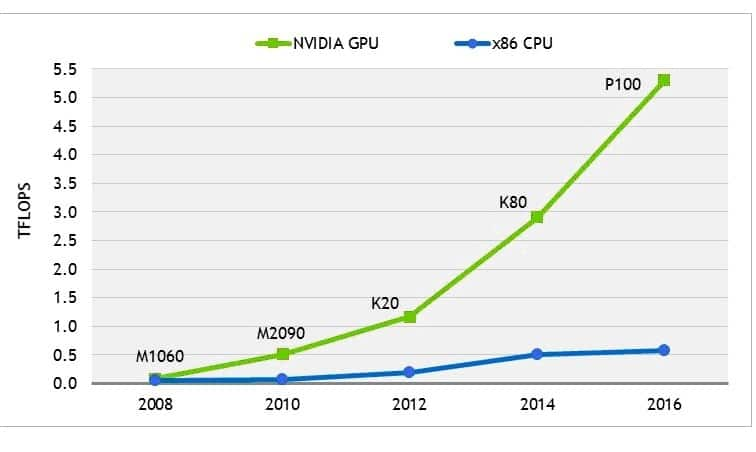
\includegraphics[scale=0.4]{gpugraph.jpg}
\caption{The evolution of GPU performance.}
\url{https://www.rtinsights.com/gpus-the-key-to-cognitive-computing/}
\label{f:graph}
\end{figure*}

It is through the application of deep learning techniques, that these obstacles can be overcome. Some contemporary examples of technologies, where these techniques have been applied are Nvidia's Deep Learning Super Sampling (DLSS) and AMD's FidelityFX Super Resolution.


\section{Anti-aliasing and Superresolution} \label{aasr}

In this section, a brief overview will be given on the RTR techniques that benefit from deep learning, but aren't themselves deep learned technology.

\subsection{Anti-aliasing} \label{aasr:aa}

Anti-aliasing (AA) combats the issue of under sampling, which causes aliasing. Aliasing presents itself in the form of jagged pixelated edges of objects visible to the human eye. Aliasing is undesirable and the two anti-aliasing methods that are used to minimize it are spatial anti-aliasing and temporal anti-aliasing.\cite{9441822}
Spatial AA computes information from a single rendered image and then implements AA on the image. They also sample sub-pixel points to smooth out the edges that would otherwise appear pixelated.\cite{9441822}
Temporal AA uses information from previously rendered frames (temporal history) and supersampling.\cite{9441822} One disadvantage of temporal AA is the potential for blurred images while rapidly rendering frames that are drastically different from each other, for example in fast paced shooter video games.

\subsection{Superresolution} \label{aasr:sr}

Superresolution (SR) generates a high-resolution output image from a low-resolution reference. It is useful in lessening VRAM usage in GPUs and also increasing framerates.\cite{8723565} It is also used in AMD's FidelityFX deep learned technology.

\section{Deep Learned Technologies} \label{deep}

Deep learning solutions "combine Convolutional Neural Networks (CNNs) and temporal history to perform sampling, anti-aliasing, ray vector calculations for multiple bounces, etc. on downscaled low-resolution frames. The CNN is then used to apply superresolution on the downscaled frame. Deep learning techniques for RTR generate significantly less GPU load since the frame is being rendered at a sub-native resolution, thus allowing the GPU cores to compute scene information, present in the rendering pipeline, at a faster rate and hence enable developers to implement support for better effects and higher resolutions."\cite{9441822} This diagram in fig.~\ref{f:fsr} shows how such a deep learned technology works.

\begin{figure*}[htpb]
\centering
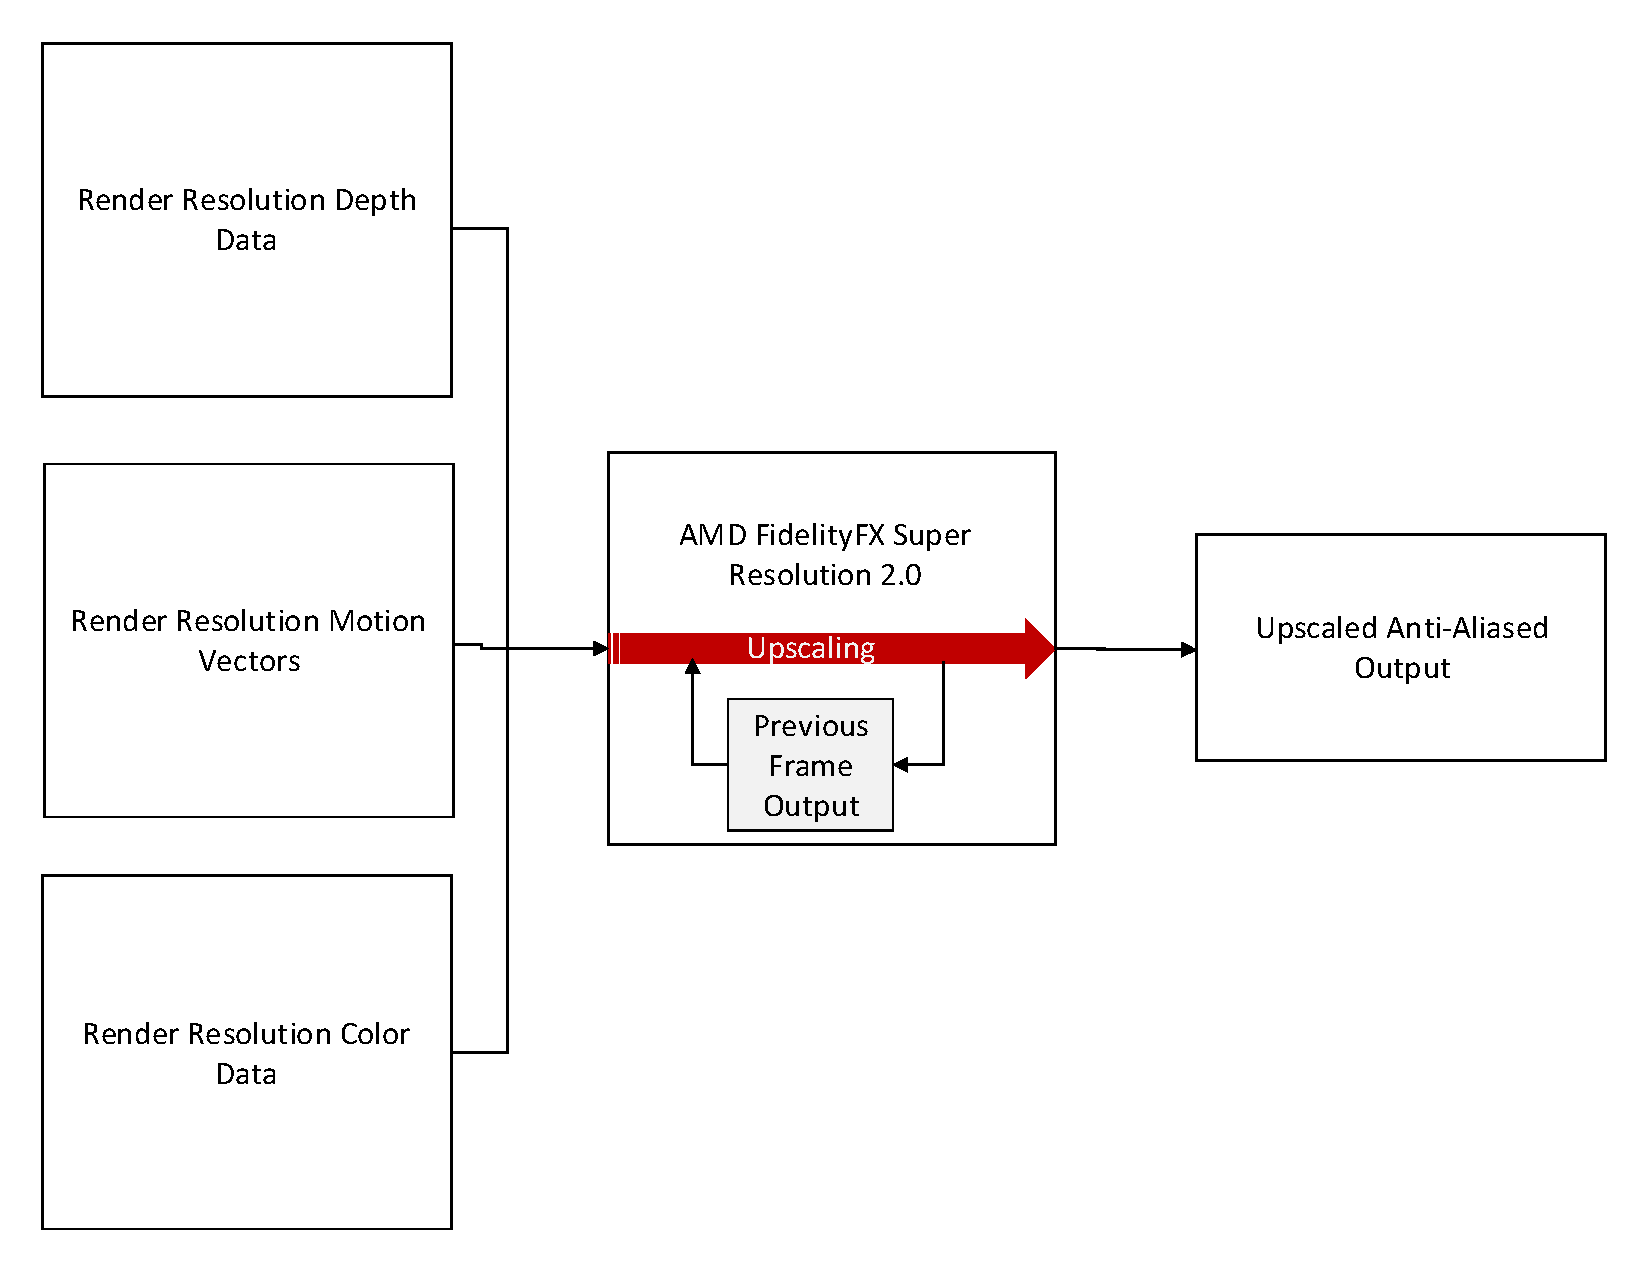
\includegraphics[scale=0.4]{diagramFSR.pdf}
\caption{Diagram of AMD FidelityFX 2.0.}
\url{https://www.amd.com/en/technologies/fidelityfx-super-resolution}
\label{f:fsr}
\end{figure*}

\subsection{Deep Learning Super Sampling} \label{deep:dlss}

Deep Learning Super Sampling or DLSS is Nvidia’s closed-source hardware-accelerated SR technique which was introduced during the GTC 2018 keynote. The most recent generations of Nvidia GPUs have dedicated AI accelerator cores called tensor cores along with the standard CUDA cores. Tensor cores are very fast dedicated image matrix multiplication circuitry where each matrix is a 16-bit floating point 4 x 4 matrix. The DLSS neural network is executed on the tensor cores.\cite{oh2018nvidia} Fig.~\ref{f:fps} shows how DLSS can improve framerates in video games.

\begin{figure*}[tbh]
\centering
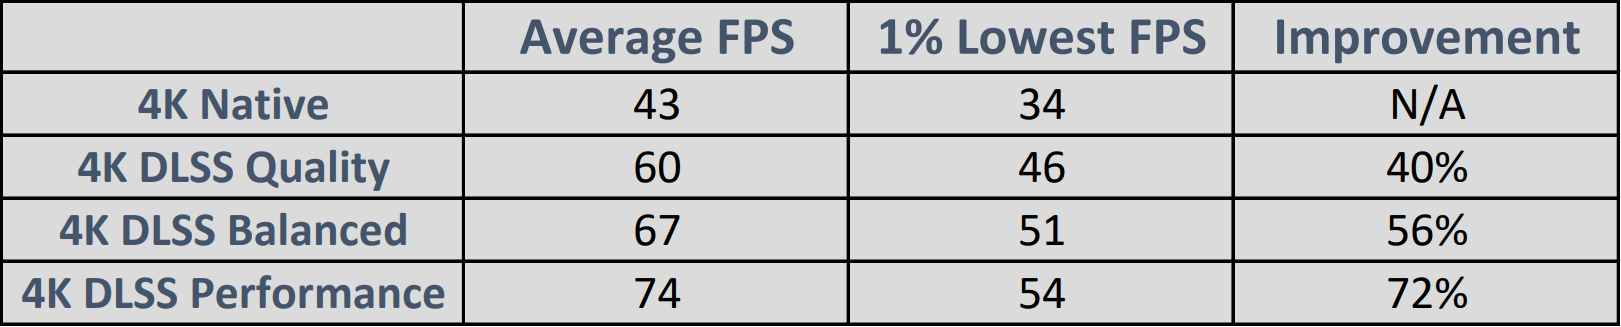
\includegraphics[scale=0.4]{FPS.png}
\caption{Table of FPS values in the game Deathloop running on an Nvidia RTX 2080 Super GPU at 4K resolution on Ultra settings.}
\label{f:fps}
\end{figure*}

\subsection{Neural Super Sampling} \label{deep:neural}

In a paper titled “Neural Supersampling for Real-time Rendering”, Xiao et al. introduced a novel SR model that requires no special proprietary hardware to execute and hence can be implemented on a wide range of existing platforms. The Neural Supersampling (NSS) model allows for 4 x 4 upsampling as compared to 2 x 2 upsampling in other SR techniques. This method utilizes common inputs from render engines such as depth maps, motion vectors and pixel colours to address the problems of high quality upsampling from low-resolution aliased input images.\cite{9441822}

\section{Challenges and potential solutions} \label{challenges}

While these technologies have achieved significant performance gains, there are still many challenges they face. Some of these techniques require significant computing power to execute, therefore they need to be simplified without negatively affecting the end result. They also need more efficient algorithms, since a large amount of information can be lost in some cases. These technologies are still in their infancy and need to be further developed and more widely implemented, so as to become more useful and gain wider support. In some exceptional cases, these technologies shouldn't be used under any circumstance without significant oversight. For example in remasters or remakes of older video games, made to look more realistic. One specific example is GTA San Andreas Remastered, where every game object was upscaled to look better, however, it had many unintended consequences, such as losing definition in deliberately polygonal shapes and misshapen, wrongly applied textures.

\section{Conclusion} \label{conclusion}

In conclusion, because real-time rendering has become more difficult, deep learned technologies definitely have a place in the gaming industry and will continue to have a bigger impact in future. However, they need to be further developed in unison with other RTR techniques and also with GPU hardware. They need to be constantly evolving and resolving any issues that may arise, but they are currently a great way to reduce the workload on the GPU and power consumption. Some of these techniques may also be applied in other fields, such as video compression\cite{9675356} or enhancing of images\cite{9792975}.

\bibliography{literatura}
\bibliographystyle{plain}
\end{document}
